\documentclass[12pt]{article}
\usepackage[english]{babel}
\usepackage[letterpaper,margin=1in]{geometry}
\usepackage[parfill]{parskip}
\usepackage{mathtools}
\usepackage{amssymb}
\usepackage{underscore}
\usepackage{hyperref}
\usepackage{graphicx}
\graphicspath{{img/}}
\frenchspacing
\author{Ariel Davis (azdavis), Jerry Yu (jyu)}
\date{\today}
\title{15-418 Final Project Proposal}
\begin{document}
\maketitle

\subsection*{Overview}
We have decided to build bokeh portrait mode in parallel.

Bokeh portrait mode has been popularized largely by DSLR cameras, where the
foreground of the subject is in focus and the background is blurred by bokeh
shapes. Up until recently, images with bokeh portrait mode had to be taken
from high end DSLR cameras that cost up to thousands of dollars. But now,
portrait mode has been integrated into smartphones, with the foreground
detection and blur done mainly with image processing. (Google Pixel 2) Many
smartphones in the market currently use multiple cameras (IPhone X) for
depth detection but our project will focus on the image processing method.

Portrait mode can be seperated into two main steps. The first is the segment
the given image into a foreground and background. Segmentation is done in order
to replicate the DSLR camera being able to capture foregrounds in focus and
backgrounds out of focus.
The second is the bokeh blur, which is applied to the background parts of the
image. A bokeh blur must be calculated with a polygon, in order to replicate the
fractions of light let through the specific apertures a DSLR camera.

We believe that parallelism can be utilized in both of these steps. For the
blur, the entire region can be entirely completed in parallel as there are
little dependencies after the blur process. Depending on which segmentation
algorithm we utilize (options explained in next section), we will also
implement it in parallel to achieve speedup.

\subsection*{Part 1: Segmentation}
There are several different implementations of foreground/background removal
and extraction algorithms. In order to maximize parallelism and due to our lack
of knowledge for machine learning, we will focus on classic computer vision
methods rather than identifying foreground with convolutional neural nets
\cite{pixel-ml}.

Some of the main algorithms we have looked at are active contour methods
(snake), principle component analysis, and graph cut algorithms.

We will most likely implement the active contour method, as it is the easiest
to implement. The algorithm uses a spline known as a snake that is influenced
by energy values in the image calculated by the pixel values. Essentially,
snakes start from the outside of an image as a line and try to continue towards
the center. If it believes there is not that large of a pixel difference with
what it has seen previously, it proceeds towards the center. Otherwise, it
stops because it believes it has reached the foreground of the image.

In terms of computation, a gradient of the pixels must be first calculated in
order to find differences in pixel values. This gradient can be heavily parallelized with
CUDA. The gradient is then used in order to calculate lines and edges in the
images, which are contours that the snake uses to determine its energy and
the energy of the pixels in the image. The energy is then used to make
decisions for the points of a snake.

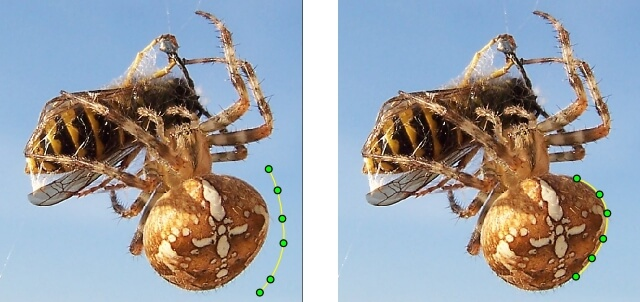
\includegraphics{snake-contour-example.jpg}
\cite{contour-model}

Each point of the snake has its own energy and the decision to move the point
is independent to the other points of the snake, so there is opportunity to
utilize parallelism. OpenMP can be utilized here if there are around 12 points
used in the snake.

\subsection*{Hardware}
We will use the gates machines, as they have GPUS if we use CUDA and a high
number of hyperthreads for OMP processing.

\begin{thebibliography}{999}
\bibitem{pixel-ml}
\href
{https://research.googleblog.com/2017/10/portrait-mode-on-pixel-2-and-pixel-2-xl.html}
{Google Research - Portrait Mode}
\bibitem{contour-model}
\href
{https://en.wikipedia.org/wiki/Active_contour_model}
{Active contour model}
\end{thebibliography}
\end{document}
